
\chapter{Fundamentação Teórica\label{chap:FundamentacaoMatematica}}

% Resumo opcional. Comentar se não usar.
\resumodocapitulo{Opcional, geralmente se colocam pequenos resumos
ou citações que se achar relevantes.}


\section{Introdução}

Este capítulo irá apresentar algumas soluções para o problema de tomada de decisões em sistemas de robótica móvel encontradas em outros trabalhos anteriores nessa área. Será abordado, também, o problema de aprendizagem por reforço e algumas alternativas de como é executado na literatura. Por último, esse capítulo irá introduzir a teoria matemática por trás dos algoritmos utilizados nesse projeto.


\section{Revisão Bibliográfica} \label{section:RevisaoBibliografica}

Aqui iremos descrever diferentes abordagens encontradas na literatura para o problema de tomada de decisões aplicado a sistemas de robótica móvel. A tomada de decisões é um problema de amplo espectro para o qual existem várias estratégias diferentes que tentam solucioná-lo.

Analisando a literatura, podemos ver a preferência crescente por algoritmos probabilísticos nessa área, no lugar dos determinísticos. Isso provem da incerteza presente no mundo real, que deve ser modelada pelo algoritmo adotado. Para uma modelagem verdadeira e precisa do mundo real, é preciso considerar as incertezas presentes nele.

Muitos algoritmos de planejamento de tarefas são específicos para as tarefas que seus robôs irão desempenhar, alguns exemplos são na área de exploração, por exemplo, o uso de algoritmos de exploração de fronteiras [4, 5, 6] ou na área de braços robóticos para planejamento de manipulação de objetos para robôs com dois braços [7].

Para o nosso sistema queríamos um algoritmo que não fosse específico para um único tipo de aplicação. Analisando a literatura mais a fundo, vemos que muitos algoritmos nessa área são baseados na cadeia de Markov. Ela diz que o ambiente pode ser modelado por um número de variáveis de estado em que cada estado depende apenas do estado exatamente anterior ( $ P(S^t\mid S^{t-1}S^{t-2})=P(S^t\mid S^{t-1}) $ ), ou seja, o sistema não tem memória de longo prazo [8].

Um algoritmo baseado na cadeia de Markov que é muito utilizado é o Processos de Decisão de Markov (Markov Decision Processes, MDP) [3]. Um problema desse algoritmo é que, embora ele leve em conta que as ações executadas podem ter um comportamento imprevisível, ele não incorpora a incerteza provinda dos sensores. Em outras palavras ele considera que o estado do sistema pode ser completamente observado a todo instante, o que, em robótica, geralmente não é o caso.

Um algoritmo que corrige esse problema é o Processos de Decisão de Markov Parcialmente Observável (Partially Observable Markov Decision Processes, POMDP) [3]. Esse algoritmo retorna para o caso geral completamente probabilístico em que ambos os sensores e os atuadores tem funcionamento imprevisível e com certa curva conhecida de probabilidade. O problema com esse algoritmo é a sua demanda computacional, mesmo podendo ser calculado off-line e salvo, ele muitas vezes não é computacionalmente possível.

Em [9] Pineau e Thrun utilizam uma estratégia de vários POMDPs hierarquizados para reduzir o problema de requisição computacional que um único POMDP combinado iria precisar.

Outra estratégia para o planejamento de tarefas é uma estratégia reativa baseada na seleção de comportamentos presente em [1, 10]. Essa é uma estratégia interessante, pois, computacionalmente ela é eficiente, ao se selecionar somente um comportamento e posteriormente se escolher uma ação para ele, consegue-se reduzir consideravelmente as opções a se tomar (existem menos comportamentos do que ações possíveis). Essa estratégia foi expandida posteriormente em [11] para se aprender a os modelos probabilísticos de seleção de comportamentos a partir de entradas humanas.

Na área de aprendizagem de modelos ou de políticas para execução de ações, existem vários algoritmos baseados no MDP citado acima. Alguns deles, que focam apenas na aprendizagem do modelo [refs Model learning] tem várias aplicações, sendo análise de mercados para economia uma delas [refs Model learning calvet]. Outro exemplo de algoritmo de aprendizagem é o de diferença temporal, que é utilizado para avaliar uma dada política%
\footnote{Uma política pode ser vista como uma função $ \pi \left( S \right) $, a qual, dado um estado, retorna uma ação possível de ser executada nele%
}
[refs temporal difference, q learning book].

Outras estratégias de aprendizagem por reforço permitem aprender uma política ótima de comportamentos ou ações para um dado agente. Uma delas é o Q Learning [refs q learning book, q learning], que é um algoritmo simples, mas eficiente, que aprende valores de ganho para cada par ação-estado, e com isso consegue alcançar uma política ótima. Outro algoritmo importante é o ator crítico [refs reinforcement learning book, actor crictic], que aprende uma política ótima ao separar um ator, o qual escolhe essa política, e um crítico, que avalia a política e provê um feedback para o ator.

Nesse trabalho nós criaremos uma nova abordagem, baseada em [1, 10], para fazer uma seleção de comportamento e ação para um agente móvel com sensores probabilísticos. Além disso, utilizaremos o algoritmo de aprendizagem por reforço q learning, presente em [ref reinforcement learning book], para aprender uma política ótima de escolha de comportamento.


\section{Filtro Bayesiano} \label{section:FiltroBayesiano}

Um filtro bayesiano é uma abordagem probabilística para estimar uma função de densidade de probabilidade desconhecida de forma recursiva no tempo, utilizando ações e observações, além de um modelo matemático do processo.

No filtro bayesiano nós queremos obter a distribuição conjunta de probabilidade:

\begin{equation}
	P ( M^{0: t} S^{0: t} Z^{0: t} \mid \pi_f )
\end{equation}

Sendo $ M^i $ o conjunto de ações no tempo $ i $, $ S^i $ o estado do sistema nesse instante e $ Z^i $ os dados dos sensores, também nesse instante. Essa função de probabilidade representa a probabilidade de uma sequência de ações, observações e estados acontecerem dado o que se sabe sobre o mundo ($ \pi_f $). Para obter esse valor tiraremos proveito das propriedades desse sistema que é baseado numa cadeia de Markov%
\footnote{Como explicado na seção \ref{section:RevisaoBibliografica}, a probabilidade de se alcalnçar um estado $ s^t $ no instante de tempo $ t $, dado que se conhece o estado $ s^{t-1} $, independe de $ s^{t-2} $. $ P(S^t\mid S^{t-1}S^{t-2})=P(S^t\mid S^{t-1}) $%
}%
.

\begin{equation}
        P ( M^{0: t} S^{0: t} Z^{0: t} \mid \pi_f ) = P ( M^0 S^0 Z^0 \mid \pi_f ) \cdot \prod\limits_{j =1}^{t} 
        \left(
            \begin{array}{l}
                P( S^j \mid S^{j -1} M^{j -1} \pi_f ) \\
                \times P( Z^j \mid S^j \pi_f ) \\
                \times P( M^j \mid S^j M^{j -1} \pi_f )
            \end{array}
        \right)
\end{equation}

Essa equação explicita quatro itens:

\begin{itemize}
  \item $ P \left( M^0 S^0 Z^0 \mid \pi_f \right) $ : As probabilidades do estado inicial do sistema são necessárias para se obter seus futuros valores;
  \item $ P \left( S^j \mid S^{j-1} M^{j-1} \pi_f \right) $ : Cada estado depende do estado anterior e de que ação foi tomada (termo de predição);
  \item $ P \left( Z^j \mid S^j \pi_f \right) $ : É necessário um modelo de probabilidades do sensor. Esse termo representa a probabilidade de se ter recebido uma certa medida dos sensores, dado que o estado atual realmente seja $ S^j $ (termo de observação)
  \item $ P \left( M^j \mid S^j M^{j-1} \pi_f \right) $ : A escolha da próxima ação depende de qual o estado do sistema e qual foi a ação anterior (termo de decisão de ação)
\end{itemize}

\begin{figure}[h]
    \centering
    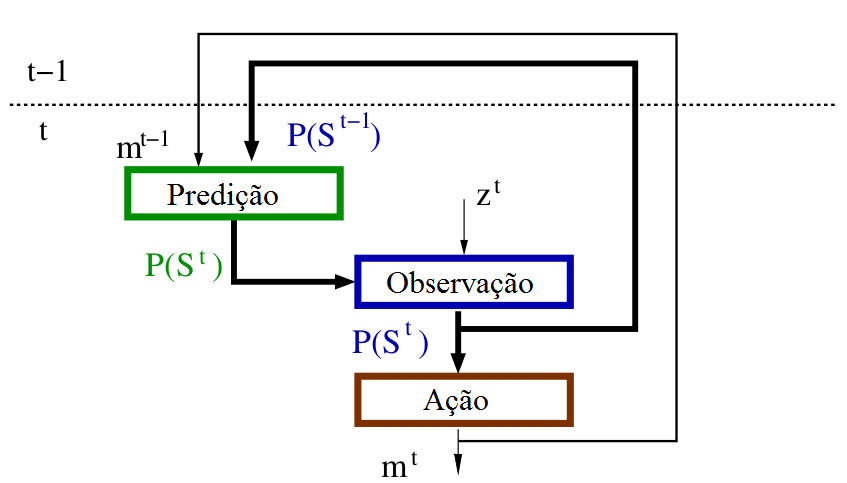
\includegraphics[width=120mm]{images/modelo_bayesiano-carla}
    \caption{\label{img:ModeloProbabilisticoCarla}Filtro Bayesiano Recursivo. Fonte: \cite{INCA2005} [Trocar por tese da Carla]}
\end{figure}

Com essas densidades probabilísticas podemos decidir por uma estratégia de ação em qualquer instante de tempo utilizando a ação $ M^t = m $ que maximize essa função. Podemos também descobrir o estado mais provável de o sistema se encontrar fazendo a mesma coisa para $ S^j $.

Esse modelo pode, ainda, ser discretizado para cada instante de tempo, ficando:

\begin{equation}
        P ( M^{0: t} S^{0: t} Z^{0: t} \mid \pi_f ) = P ( M^{0: t-1} S^{0: t-1} Z^{0: t-1} \mid \pi_f ) \cdot 
        \left(
            \begin{array}{l}
                P( S^j \mid S^{j -1} M^{j -1} \pi_f ) \\
                \times P( Z^j \mid S^j \pi_f ) \\
                \times P( M^j \mid S^j M^{j -1} \pi_f )
            \end{array}
        \right)
\end{equation}

Com isso temos um modelo recursivo que pode ser chamado a cada instante de tempo para atualizar o modelo de probabilidades. Essa atualização pode ainda ser dividida em três partes distintas:

\subsection{Predição}

Nessa etapa, a partir da ação escolhida no período anterior de tempo, se faz uma estimativa de qual será o estado após sua execução.

\begin{equation}
    P \left( S^t \mid z^{0: t-1} m^{0: t-1} \pi_f \right) \propto \sum\limits_{S^{t-1}}
        \left(
            \begin{array}{l}
                P \left( S^t \mid S^{t-1} m^{t-1} \pi_f \right) \\
                \times P \left( m^{t-1} \mid S^{t-1} m^{t-2} \pi_f \right)\\
                \times P \left( S^{t-1} \mid z^{0: t-1} m^{0: t-2} \pi_f \right)
            \end{array}
        \right)
\end{equation}


\subsection{Observação}

Tendo, agora, um dos comportamentos escolhido, se atualiza o belief state do agente a partir dos sensores presentes no robô.

\begin{equation}
    P \left( S^t \mid z^{0: t} m^{0: t-1} \pi_i \right) \propto 
        \left(
            \begin{array}{l}
                P \left( z^t \mid S^t \pi_f \right) \\
                \times P \left( S^t \mid z^{0: t-1} m^{0: t-1} \pi_f \right)
            \end{array}
        \right)
\end{equation}


\subsection{Escolha de ação motor}

Por último se faz a seleção de uma ação a ser executada pelo robô de forma análoga à seleção de comportamentos. Calcula-se as probabilidade de se executar cada ação  e se escolhe a com maior valor.

\begin{equation}
    P \left( M^t \mid z^{0: t} m^{0: t-1} \pi_f \right) \propto \sum\limits_{S_i^t}
        \left(
            \begin{array}{l}
                \times P \left( M^t \mid S^t m^{t-1} \pi_f \right)\\
                \times P \left( S^t \mid z^{0: t} m^{0: t-1} \pi_f \right)
            \end{array}
        \right)
\end{equation}


\section{MDP (Processo de Decisão de Markov)} \label{section:MDP}

MDPs são utilizados em várias áreas, como economia, manufatura de processos e robótica. Ele foi nomeado a partir de Andrey Markov e provê uma base matemática para o modelamento de tomada de decisões. Eles são uma extensão de cadeias de Markov, tendo como diferença a adição de ações e recompensas (escolha e motivação).

MDP é, mais precisamente, um processo de controle estocástico de tempo discreto. O que isso significa é que ele é um processo de controle probabilístico, baseado em passos (time steps). Em cada passo o robô se encontra em um estado $ S $ perfeitamente conhecido em que pode-se executar qualquer ação $ u $ disponível para esse estado. O modelo de percepção do robô, $ p \left( Z \mid S \right) $ é uma equação determinística e bijetora, o robô só pode estar em um estado $ s \in S $ para uma percepção $ z \in Z $ do ambiente.

Após executada essa ação, o robô se encontrará em um novo estado $ s' \in S $ com probabilidade $ p \left( s' \mid u, s \right) $, essa equação é conhecida como modelo de atuação (action model). O modelo de atuação não é, em geral, determinístico, ou seja, uma ação pode ter várias consequências com diferentes probabilidades. Uma consequência disso é que planejar uma única sequência de ações não é o suficiente, o planejador de decidir por uma ação para cada um de uma gama de estados em que o robô pode se encontrar.

Considere o sistema de figura a seguir em que para uma dada ação A ou B tem-se indicada as probabilidades $ p \left( s' \mid u, s \right) $ através da percentagem indicada nas setas saindo do estado $ s $ para $ s' $.


\begin{figure}[h]
    \centering
    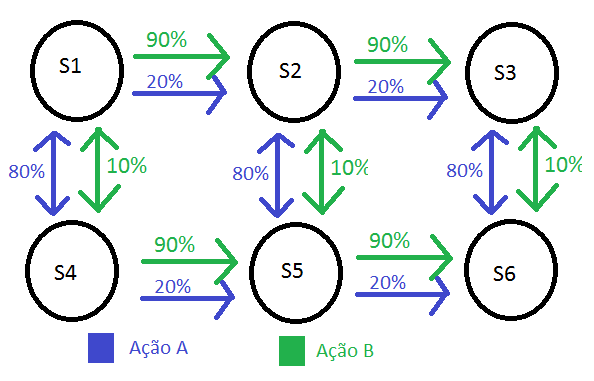
\includegraphics[width=120mm]{images/probabilidade-markov}
    \caption{\label{img:MapaDeProbabilidadesMarkov}Mapa de Probabilidades}
\end{figure}

Podemos, por exemplo, ver que para esse sistema $ P \left( s2 \mid a, s1 \right) = 0.2 $ e $ P \left( s4 \mid a, s1 \right) = 0.8 $. Se nós tivermos o estado $ s6 $ como objetivo, note que não adianta se obter uma sequência de ações $ a \rightarrow a \rightarrow b$, por exemplo, pois nós podemos nos encontrar em uma gama de estados ao final dessa sequência. Poderíamos nos encontrar em $ s4 $, $ s2 $ ou $ s6 $.

Temos então de mapear uma ação para cada estado possível em que pudermos nos encontrar, gerando o que é chamado de política de controle (control policy). Essa política de controle terá formato $ \pi: S_t \rightarrow U_t $, a política $ \pi $ recebe um estado e retorna a ação planejada para ele. Note então que, tendo essa política $ \pi \left( S \right) $, não temos problemas como no caso anterior, pois sempre teremos planejado que ação tomar em um dado instante, baseado no estado em que nos encontrarmos.

Calcular essa política não é um problema trivial, devido, entre outros motivos, à existência de infinitos caminhos para se chegar de um estado $ s1 $ a $ s6 $. Um caminho seria $ s1 \rightarrow s2 \rightarrow s3 \rightarrow s6 $, por exemplo, e outro seria $ s1 \rightarrow s2 \rightarrow s5 \rightarrow s2 \rightarrow s3 \rightarrow s6 $, outro ainda seria $ s1 \rightarrow s2 \rightarrow s5 \rightarrow s2 \rightarrow s5 \rightarrow s2 \rightarrow s3 \rightarrow s6 $.

Antes de poder obter um algoritmo definitivo, temos de modelar o que seria o objetivo de um problema. Para isso utilizaremos uma função de recompensa para o robô $ r \left( S, U, S' \right) $ que retorna um número real. Ela indica quão desejado é se chegar a uma estado $ s' $ a partir de $ s $ executando a ação $ u $. Para sistemas em que só se preocupe em chegar ao estado desejado pode-se simplifica-la para $ r \left( s' \right) $, por exemplo.

Sabendo que queremos achar uma política que maximize o ganho de recompensas podemos gerar um plano de políticas ótimo pensando-se apenas na próxima ação, maximizando uma recompensa imediata. Caso nossas recompensas fossem dadas apenas pela escolha de uma ação baseada no estado atual $ r \left( S, U \right) $ (sem considerar o estado alcançado) teríamos como escolha de política:

\begin{equation}
    \pi_1 \left( s \right) = \underset{u}{argmax} \left( r \left( s, u \right) \right)
\end{equation}

Como nossa recompensa depende também do estado alcançado, devemos pesar cada recompensa $ r \left( S, U, S' \right) $ pela probabilidade de se alcançar o estado $ S' $.

\begin{equation}
    \pi_1 \left( s \right) = \underset{u}{argmax} \left( \int \! r \left( s, u, s' \right) \cdot P \left( s' \mid u, s \right) \, \mathrm{d}s'. \right)
\end{equation}

Podemos gerar para essa política um função de valor (value function) que represente a recompensa esperada para cada estado $ s $ seguindo a política $ \pi $.

\begin{equation}
    V_1 \left( s \right) = \underset{u}{max} \left( \int \! r \left( s, u, s' \right) \cdot P \left( s' \mid u, s \right) \, \mathrm{d}s'. \right)
\end{equation}

Pensando no passo seguinte, podemos utilizar esse novo valor $ V_1 \left( S \right) $ para calcular uma política planejando agora um passo à frente e depois generalizar para qualquer caso futuro.

\begin{equation}
    \pi_t \left( s \right) = \underset{u}{argmax} \left( \int \! \left( r \left( s, u, s' \right) + \gamma \cdot V_{t-1} \left( s' \right) \right) \cdot P \left( s' \mid u, s \right) \, \mathrm{d}s'. \right)
\end{equation}

Sendo $ \gamma $ uma constante de desconto, usada para incentivar o ganho de recompensas imediatas à tardias. Essa função indica que a política ótima é a que gera uma maior recompensa imediata, somada com a somatória de todas as recompensas futuras esperadas ponderadas pelas probabilidades de serem recebidas. Podemos novamente gerar uma função de valor para essa política:

\begin{equation}
    V_t \left( s \right) = \underset{u}{max} \left( \int \! \left( r \left( s, u, s' \right) + \gamma \cdot V_{t-1} \left( s' \right) \right) \cdot P \left( s' \mid u, s \right) \, \mathrm{d}s'. \right)
\end{equation}

Para um tempo $ t = \infty $, a política geralmente converge e uma ótima para esse sistema é encontrada.

\begin{equation}
    \pi^* \left( s \right) = \pi_\infty \left( s \right) = \underset{u}{argmax} \left( \int \! \left( r \left( s, u, s' \right) + \gamma \cdot V_\infty \left( s' \right) \right) \cdot P \left( s' \mid u, s \right) \, \mathrm{d}s'. \right)
\end{equation}

\begin{equation} \label{equation:ValueFunctionMDP}
    V^* \left( s \right) = V_\infty \left( s \right) = \underset{u}{max} \left( \int \! \left( r \left( s, u, s' \right) + \gamma \cdot V_\infty \left( s' \right) \right) \cdot P \left( s' \mid u, s \right) \, \mathrm{d}s'. \right)
\end{equation}


\section{TD (Diferença Temporal)} \label{section:TD}

O que fazer se você não conhece os valores das recompensas $ r \left( S, U, S' \right) $ ou qual o resultado de uma ação $ P \left( s' \mid u, s \right) $? O algoritmo de diferença temporal visa, a partir de uma política fixa $ \pi \left( S \right) $, aprender os valores finais de $ V \left( S \right) $ através da execução de ações em diferentes estados, sem ter um conhecimento prévio das recompensas recebidas ou do modelo probabilístico do resultado de suas ações.

Esse algoritmo se baseia na equação \ref{equation:ValueFunctionMDP} obtida no seção \ref{section:MDP} e parte da premissa de que se tem uma política $ \pi_{td} $ já escolhida e fixa. Utilizando isso ele atualiza o valor de $ V \left( S \right) $ cada vez que experiencia um $ \left( s, u, s', r \right) $ qualquer, ou seja, que alcança um estado $ s' \in S $ a partir do estado $ s \in S $, com uma ação $ u \in U $ e recebendo uma recompensa $ r \in \mathbb{R} $. A partir de cada dessas experiências, pode-se obter um valor amostra tal que:

\begin{equation} \label{equation:AmostraTD}
	amostra = r \left( s, u, s' \right) + \gamma \cdot V_{\pi_{td}}^t \left( s' \right)
\end{equation}

Agora, escolhendo-se uma constante de aprendizagem $ \alpha $, pode-se atualizar o valor de $ V_{\pi_{td}} \left( s \right) $ tal que:

\begin{equation} \label{equation:UpdateValueFunctionTD}
	V_{\pi_{td}}^t \left( s \right) = \left( 1 - \alpha \right) \cdot V_{\pi_{td}}^{t-1} \left( s \right) + \alpha \cdot amostra
\end{equation}

Note que, utilizando valores suficientemente pequenos de $ \alpha $, consegue-se valores de $ V_{\pi_{td}} \left( s \right) $ que convergem com o tempo e que, mais importante, convergem para os mesmos valores que o algoritmo MDP, considerando que a política $ \pi_{td} $ utilizada é ótima.

O problema com a diferença temporal é que ela apenas avalia uma política fixa e já existente. Caso queiramos mudar nossa política, ou gerar uma utilizando esse algorítmo, teríamos um problema, todos os valores de $ V \left( S \right) $ dependem somento do estado e não da ação executada. Caso se mudasse a política $ \pi_{td} $ executada, teríamos de recalcular todos os valores $ V \left( S \right) $.

\section{Q Learning} \label{section:QLearning}

Q Learning é um dos mais conhecidos e mais utilizados algoritmos de aprendizagem por reforço, sendo utilizado para controle de robôs [adicionar ref], tratamento de problemas em processamento de imagens [adicionar ref] e criação de sistemas de troca financeiros [adicionar ref]. Esse é um algoritmo, diferentemente do TD, de aprendizagem ativa, ou seja, a escolha da política e das ações é feita juntamente com a aprendizagem e se consegue alcançar uma nova política ótima o utilizando.

Ao invés de utilizar o valor de $ V \left( S \right) $ e se basear na equação \ref{equation:ValueFunctionMDP}, ele utiliza um valor $ Q \left( S, U \right) $, tal que:

\begin{equation} \label{equation:PolicySelectionQLearning}
    \pi^t \left( s \right) = \underset{u}{argmax} \left( Q^t \left( s, u \right) \right)
\end{equation}

\begin{equation}
    V^t \left( s \right) = \underset{u}{max} \left( Q^t \left( s, u \right) \right)
\end{equation}

Ou seja:

\begin{equation} \label{equation:QValueFunctionQLearning}
    Q^t \left( s, u \right) = \int \! \left( r \left( s, u, s' \right) + \gamma \cdot V^{t-1} \left( s' \right) \right) \cdot P \left( s' \mid u, s \right) \, \mathrm{d}s'
\end{equation}

Que pode ser reescrito como:

\begin{equation} \label{equation:QValueFunctionQLearningFinal}
    Q^t \left( s, u \right) = \int \! \left( r \left( s, u, s' \right) + \gamma \cdot \underset{u'}{max} \left( Q^{t-1} \left( s', u' \right) \right) \right) \cdot P \left( s' \mid u, s \right) \, \mathrm{d}s'
\end{equation}

Ao aprender o valor de $ Q^t \left( S, U \right) $, ao invés do de $ V^t \left( S \right) $, você pode modificar sua política sem ter que reaprender todos os seus valores. Analogamente às equações \ref{equation:AmostraTD} e \ref{equation:UpdateValueFunctionTD} em TD, aprende-se através de amostras obtidas a partir de experiências $ \left( s, u, s', r \right) $.

\begin{equation} \label{equation:AmostraQLearning}
	amostra = r \left( s, u, s' \right) + \gamma \cdot \underset{u}{max} \left( Q^{t-1} \left( s', u' \right) \right)
\end{equation}

\begin{equation} \label{equation:QUpdateQLearning}
	Q^t \left( s, u \right) = \left( 1 - \alpha \right) \cdot Q^{t-1} \left( s, u \right) + \alpha \cdot amostra
\end{equation}

Com um número suficiente de iterações e com um decaimento apropriado do parâmetro de aprendizagem $ \alpha $, $ Q^t \left( S, U \right) $ tende a um valor ótimo  com uma probabilidade 1 [adicionar refs convergência de q] e uma política escolhida com base na função \ref{equation:PolicySelectionQLearning} também seria ótima.

Alguns problemas com esse algoritmo são:

\begin{itemize}
	\item Podem existir muitos estados para se visitar, para um espaço contínuo, por exemplo, seriam infinitos;
	\item Podem existir muitas ações possíveis para cada estado, para o acionamento analógico de um motor, por exemplo, seriam infinitas;
	\item Se houverem muitos pares ação-estado $ \left( S, U \right) $, mesmo que se consiga aprender por um tempo muito grande, tem que se conseguir armazenar o valor de $ Q_t \left( S, U \right) $ para cada ação que for possível de ser executada em cada estado;
	\item O algoritmo não consegue aplicar o que aprendeu em um estado para outros com características parecidas.
\end{itemize}

\subsection{Generalização dos Pares Estado-Ação} \label{subsection:GeneralizaçãoParesEstadoAção}

Uma solução para esse problema é generalizar a informação de um par estado-ação para outros similares. Para isso utilizaremos um vetor de características $ f $ para descrever o estado. Essas características podem ser coisas como:

\begin{itemize}
	\item Distância para uma posição que oferece uma recompensa positiva;
	\item Distância para uma posição que oferece uma recompensa negativa;
	\item Número de alvos a serem capturados;
	\item Estado do robô (Com ou sem problema).
\end{itemize}

Elas também podem descrever a ação a ser executada, como:

\begin{itemize}
	\item Fica parado;
	\item Move uma garra;
	\item Economiza energia.
\end{itemize}

Essas características podem até descrever um estado futuro $ s' $ (possivelmente utilizando alguma das características descritas acima) que tenha alta chance de ser alcançado por esse par estado-ação.

Podemos utilizar esse vetor de características $ f_j \left( S, U \right) $ para obter um valor $ Q \left( S, U \right) $ tal que:

\begin{equation} \label{equation:QValueGeneralizado}
	Q \left( S, U \right) = \omega_1 \cdot f_1 \left( S, U \right) + \omega_2 \cdot f_2 \left( S, U \right) + \cdots + \omega_n \cdot f_n \left( S, U \right)
\end{equation}

Com essa equação conseguimos um valor parecido de $ Q \left( S, U \right) $ para estados distintos que possuam características $ f_j \left( S, U \right) $ com valores parecidos. A desvantagem é que devemos escolher esses valores/características com cuidado para obter uma boa representação do nosso par estado-ação a partir deles, ou podemos ter estados-ações com valores de $ f_j \left( S, U \right)$ parecidos, e, consequentemente, valores de $ Q \left( S, U \right) $ também parecidos, mas que são muito diferentes.

Com esse novo modelo, podemos aprender valores, a partir de cada experiência, utilizando o erro atual do modelo:

\begin{equation}
	erro = r \left( s, u, s' \right) + \gamma \cdot \underset{u}{max} \left( Q^{t-1} \left( s', u' \right) \right) - Q^{t-1} \left( s, u \right)
\end{equation}

Dada pela diferença entre a recompensa recebida somada com o valor de ganho esperado para o novo estado alcançado e o valor atual esperado para o par estado-ação executada. E o utilizando para atualizar cada um dos pesos usados para obter $ Q_t \left( S, U \right) $:

\begin{equation}
	\omega_i^t = \omega_i^{t-1} + \alpha \cdot erro \cdot f_i \left( s, u \right)
\end{equation}

Assim, caso tenhamos um erro grande para um dado estado, iremos atualizar os valores de todos os estados com características similares àquele. É importante notar também que, caso esse estado tenha um valor maior para uma das características $ f_j $, o peso dela, $ \omega_j $, será mais modificado que os da outras características.

Note que a função utilizada para calcular $ Q \left( S, U \right) $ é um perceptron e que esse tipo de função possuí limitações, sendo a principal a de ser capaz de aprender apenas problemas linearmente separáveis [ref perceptron limitations]. Por isso os parâmetros $ f_i \left( S, U \right) $ devem ser bem escolhidos, não só para caracterizar bem um estado e permitir uma boa diferenciação entre dois deles, mas também para permitir essa aprendizagem.

\subsection{Escolha de Ações e Exploração Gulosa} \label{subsection:EscolhaDeAçõesExploraçãoGulosa}

Utilizando a equação \ref{equation:PolicySelectionQLearning}, em conjunto com \ref{equation:QValueGeneralizado}, podemos criar uma política $ \pi $ para escolha de ações. Essa política, caso o valor de $ Q \left( S, U \right) $ já tenha sido aprendido com sucesso, será ótima.

Mas, caso desde o começo do aprendizado se utilize apenas esse método para escolher a ação executada, pode se ficar preso em máximas locais%
\footnote{Uma política de ação que é melhor do que outras com pequenas variações, mas, caso se mude mais os parâmetros, existem outras melhores.%
}, sem explorar outras opções de ação. Um meio de evitar esse problema é utilizar outros métodos de exploração durante o treinamento, que podem ser desativados quando o treinamento acabar. 

Um desses métodos é chamado de exploração gulosa (\textit{greedy exploration}). É um método bem simples em que antes de se selecionar uma ação se ``arremessa uma moeda'', dependendo do resultado você ou executa uma ação randômica ou seleciona uma ação baseado no valor de $ Q^t \left( S, U \right) $ atual.

\begin{algorithm}[H]
	\caption{Exploração Gulosa} \label{euclid}
	\begin{algorithmic}[1]
		\Procedure{PegarAcao}{}
			\State $\textit{numero\_randomico} \gets \text{random }\textit{numero}$
			\If {$\textit{numero\_randomico} < \text{FATOR\_DE\_EXPLORACAO} $ }
				\State \Return $\textit{acao\_randomica}$
			\Else
				\State \Return $\textit{acao\_aprendida}$
			\EndIf
		\EndProcedure
	\end{algorithmic}
\end{algorithm}

Note que esse parâmetro $ \gamma = \textit{FATOR\_DE\_EXPLORACAO} $ é muito importante e deve ser bem escolhido. Um valor mais baixo dele limita a exploração, enquanto um mais alto atrasa a aprendizagem e pode impedir a aprendizagem de uma política que execute uma sequência de ações mais complexa.
